% !TeX program = pdflatex
\documentclass[tikz,border=8pt]{standalone}
\usepackage{pgfplots}\pgfplotsset{compat=1.16}
\definecolor{FigureBlue}{HTML}{2563EB}\definecolor{FigureOrange}{HTML}{EA580C}
\begin{document}
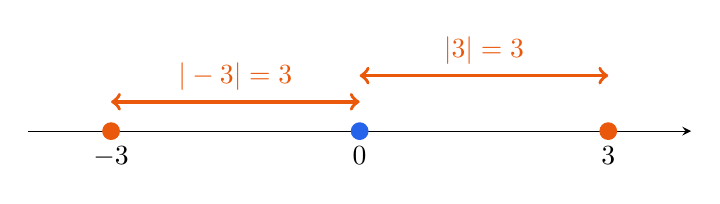
\begin{tikzpicture}
\begin{axis}[width=10cm,height=3.1cm,axis y line=none,axis x line=middle,xmin=-4,xmax=4,ymin=-.55,ymax=1,xtick={-3,0,3},ytick=\empty,clip=false]
  \addplot[only marks,mark=*,mark size=3pt,FigureBlue] coordinates {(0,0)};
  \addplot[only marks,mark=*,mark size=3pt,FigureOrange] coordinates {(-3,0)(3,0)};
  \draw[<->,FigureOrange,line width=1.3pt] (axis cs:-3,.38)--node[above] {$|-3|=3$}(axis cs:0,.38);
  \draw[<->,FigureOrange,line width=1.3pt] (axis cs:0,.72)--node[above] {$|3|=3$}(axis cs:3,.72);
\end{axis}
\end{tikzpicture}
\end{document}
